\documentclass[11pt,a4paper]{article}
\usepackage[utf8]{inputenc}
\usepackage{color}
\usepackage{enumerate}
\usepackage{fancyhdr}
\usepackage{minted}
\usepackage{graphicx}
\usepackage{array}
\usepackage{hyperref}
\usepackage{amssymb}
\usepackage[spanish]{babel}
\usepackage[spanish]{algorithm2e}

\setlength{\oddsidemargin}{18pt}
\setlength{\headheight}{14pt}
\setlength{\textheight}{609pt}
\setlength{\marginparsep}{11pt}
\setlength{\footskip}{30pt}
\hoffset = 0pt
\voffset = 0pt
\setlength{\topmargin}{0pt}
\setlength{\headsep}{25pt}
\setlength{\textwidth}{424pt}
\setlength{\marginparwidth}{54pt}
\setlength{\marginparpush}{5pt}
\paperwidth = 597pt
\paperheight = 845pt

\pagestyle{fancy}
\fancyhead[LO]{\textcolor[rgb]{0,0,0}{Grado en Ingeniería Informática}}
\fancyhead[RO]{\textcolor[rgb]{0.2,0.2,0.9}{Algorítmica, Curso 2015-2016}}

\hypersetup{
	colorlinks,
	citecolor=black,
	filecolor=black,
	linkcolor=black,
	urlcolor=black
}

\begin{document}

	\begin{titlepage}

		\centering

		\begin{figure}[h]

			\centering
			
\includegraphics[width=0.6\textwidth]{logo-ugr.png}
			
		\end{figure}

		\vspace{1cm}

		{\scshape\LARGE Universidad de Granada}

		\vspace{1cm}

		{\LARGE Algorítmica}

		\vspace{1cm}

		{\huge\bfseries\textit{Algoritmos Backtracking, parte 1}}

		\vspace{1cm}

		{\itshape\large 
		Laura Calle Caraballo \\
		Cristina María Garrido López \\
		Germán González Almagro \\
		Javier León Palomares \\
		Antonio Manuel Milán Jiménez}

		\vfill

		{\Large23 de mayo de 2016}

	\end{titlepage}

\newpage

	\tableofcontents

\newpage

	\section{Introducción.}

		\par
		El objetivo de esta práctica es el estudio de los algoritmos de tipo \textit{Backtracking}, aplicados particularmente al problema de encontrar un camino desde la entrada de un laberinto hasta su salida.

	\section{Descripción del problema.}

		\par
		Inicialmente tenemos una matriz de tamaño $n \times n$ que representa un laberinto con o sin solución. Las casillas libres se representan mediante espacios, y los muros mediante X.

		\par
		Los movimientos permitidos son: norte, sur, este y oeste (no es posible avanzar en diagonal).
	
	\section{Resolución.}

		\par
		Se han implementado dos algoritmos \textit{Backtracking}: el primero encuentra un camino (en caso de que exista) y el segundo encuentra el camino más corto posible.

		\par
		Adicionalmente, se ha realizado un estudio de eficiencia para determinar su viabilidad en términos de tiempo.

\newpage

	\section{Algoritmo \textit{Backtracking} sin garantía de optimalidad.}

		\par
		Esta versión del algoritmo construirá el camino probando diferentes alternativas hasta que encuentre una solución completa, momento en el que terminará.

		\subsection{Pseudocódigo.}

			\par
			A continuación se muestra el pseudocódigo del algoritmo:

			\vspace{2mm}

			\begin{algorithm}[H]

				posActual $\longleftarrow$ entrada\;
				camino $\longleftarrow$ camino $\cup$ posActual\;

				\textbf{function} EncontrarCamino(laberinto, posActual);

				encontrado $\longleftarrow$ false\;
				
				\Begin{

					\uIf{EsSolucion(camino)}{

						\KwRet true\;

					}

					\Else{

						\For{m $\in$ movimientosPosibles \textbf{and not} encontrado}{

							h $\longleftarrow$ GenerarHijo(m)\;

							\If{Factible(h)}{

								camino $\longleftarrow$ camino $\cup$ h\;
								encontrado $\longleftarrow$ EncontrarCamino(laberinto,h)\;

							}
						}

						\If{\textbf{not} encontrado}{

							camino $\longleftarrow$ camino $-$ posActual\;

						}
					}

					\KwRet encontrado\;

				}

			\end{algorithm}

\newpage

	\section{Algoritmo \textit{Backtracking} con garantía de optimalidad.}

		\par
		Esta versión del algoritmo encontrará un primer camino y continuará la búsqueda de un camino mejor siempre que la longitud de los recorridos que pruebe sea menor que la del mejor camino actual.

		\subsection{Pseudocódigo.}

			\par
			A continuación se muestra el pseudocódigo del algoritmo:

			\vspace{2mm}

			\begin{algorithm}[H]

				posActual $\longleftarrow$ entrada\;
				camino $\longleftarrow$ camino $\cup$ posActual\;
				mejorDistancia $\longleftarrow \infty$\;

				\textbf{function} EncontrarMejorCamino(laberinto, posActual);

				encontrado $\longleftarrow$ false\;


				\Begin{

					\uIf{EsSolucion(camino)}{

						\uIf{Longitud(camino) $<$ mejorDistancia}{

							mejorCamino $\longleftarrow$ camino\;
							camino $\longleftarrow$ camino $-$ posActual\;
							mejorDistancia $\longleftarrow$ Longitud(camino)\;
							\KwRet true\;

						}

						\Else{

							camino $\longleftarrow$ camino $-$ posActual\;
							\KwRet false\;

						}
					}

					\Else{

						\For{m $\in$ movimientosPosibles \textbf{and} Longitud(camino) $<$ mejorDistancia}{

							h $\longleftarrow$ GenerarHijo(m)\;

							\If{Factible(h)}{

								camino $\longleftarrow$ camino $\cup$ h\;
								encontrado $\longleftarrow$ EncontrarMejorCamino(laberinto,h)\;

							}
						}

						camino $\longleftarrow$ camino $-$ posActual\;

					}

					\KwRet encontrado\;

				}

			\end{algorithm}

\newpage		

	\section{Análisis de eficiencia empírico.}

		\par
		La complejidad algorítmica de estas técnicas hace que el problema sea muy costoso para dimensiones de unas pocas decenas; además, debido al proceso aleatorio de generación de laberintos, los tiempos fluctuarían mucho. Por ello, presentamos una muestra reducida y abarcable de pruebas empíricas.

		\subsection{Tabla de tiempos de ejecución.}

			\begin{figure}[h]

				\centering

				\begin{tabular}{| >{\centering\arraybackslash}m{1in} | >{\centering\arraybackslash}m{1in} | >{\centering\arraybackslash}m{1in} |}

					\hline
					\textbf{Tamaño} & \textbf{No óptimo (s)} & \textbf{Óptimo (s)} \\
					\hline
					7 & $1.57208 \cdot 10^{-11}$ & $6.21688 \cdot 10^{-11}$ \\
					\hline
					8 & $2.83452 \cdot 10^{-11}$ & $8.05098 \cdot 10^{-11}$ \\
					\hline
					9 & $7.47932 \cdot 10^{-11}$ & $2.09373 \cdot 10^{-10}$ \\
					\hline
					10 & $3.22992 \cdot 10^{-10}$ & $3.85637 \cdot 10^{-10}$ \\
					\hline
					11 & $8.27965 \cdot 10^{-10}$ & $8.49879 \cdot 10^{-10}$ \\
					\hline
					12 & $3.07938 \cdot 10^{-9}$ & $2.99815 \cdot 10^{-9}$ \\
					\hline
					13 & $5.35533 \cdot 10^{-9}$ & $3.31377 \cdot 10^{-9}$ \\
					\hline
					14 & $5.67689 \cdot 10^{-9}$ & $3.83898 \cdot 10^{-9}$ \\
					\hline
					15 & $8.04407 \cdot 10^{-9}$ & $5.83481 \cdot 10^{-9}$ \\
					\hline
					16 & $3.08026 \cdot 10^{-8}$ & $2.84645 \cdot 10^{-8}$ \\
					\hline
					17 & $5.67211 \cdot 10^{-8}$ & $2.8893 \cdot 10^{-8}$ \\
					\hline
					18 & $5.46378 \cdot 10^{-8}$ & $2.89411 \cdot 10^{-8}$ \\
					\hline
					19 & $7.24933 \cdot 10^{-8}$ & $7.94193 \cdot 10^{-8}$ \\
					\hline
					20 & $1.19869 \cdot 10^{-6}$ & $6.20915 \cdot 10^{-7}$ \\
					\hline
					21 & $2.48178 \cdot 10^{-6}$ & $1.74906 \cdot 10^{-8}$ \\
					\hline
					22 & $2.53938 \cdot 10^{-6}$ &  \\
					\hline
					23 & $5.41168 \cdot 10^{-6}$ &  \\
					\hline
					24 & $7.09637 \cdot 10^{-6}$ &  \\
					\hline

				\end{tabular}
				\caption{Tiempos de ejecución de los dos algoritmos.}

			\end{figure}

\newpage

		\subsection{Gráficas de tiempos de ejecución.}

			\par
			Podemos observar que ambos algoritmos parecen tener una tendencia de crecimiento exponencial:

			\subsubsection{Algoritmo no óptimo.}

				\begin{figure}[h]

					\centering
					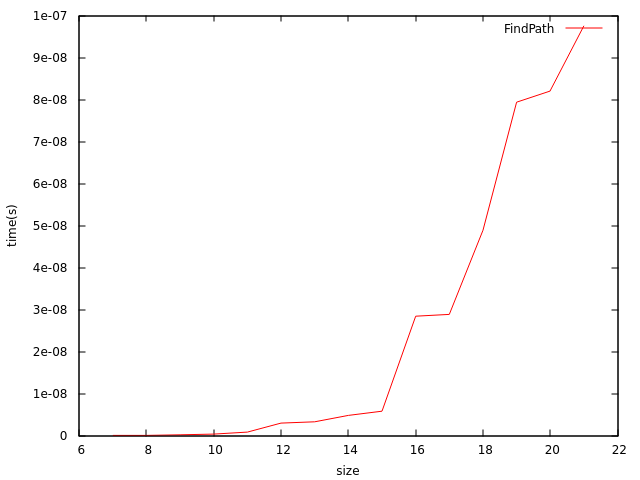
\includegraphics[width=0.59\textwidth]{FindPath.png}
					\caption{Ejecución del algoritmo que no garantiza la solución óptima. Intel® Core™ i7-5500U CPU @ 2.40GHz.}
					
				\end{figure}

			\subsubsection{Algoritmo óptimo.}

				\begin{figure}[h]

					\centering
					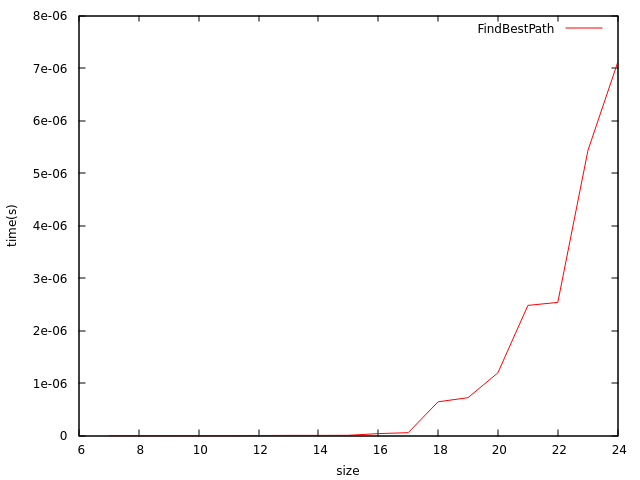
\includegraphics[width=0.59\textwidth]{FindBestPath.png}
					\caption{Ejecución del algoritmo que garantiza la solución óptima. Intel® Core™ i7-5500U CPU @ 2.40GHz.}
					
				\end{figure}

\newpage

	\section{Comparativa de calidad de soluciones.}

		\par
		Para mostrar que, efectivamente, el segundo algoritmo realiza una búsqueda más completa y encuentra caminos más cortos en caso de haberlos, compararemos las soluciones obtenidas para un caso concreto.

		\par
		El laberinto generado es el siguiente:

		\vspace{5mm}

		\begin{figure}[h]

			\centering
			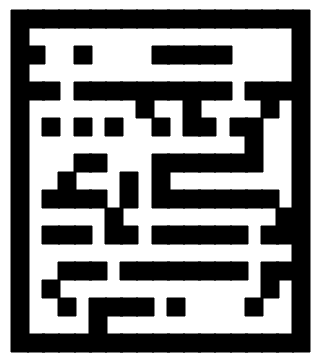
\includegraphics[width=0.6\textwidth]{Maze19.png}
			
		\end{figure}

\newpage

		\par
		La solución proporcionada por el algoritmo no óptimo tiene una longitud de 41 y es:

		\vspace{5mm}

		\begin{figure}[h]

			\centering
			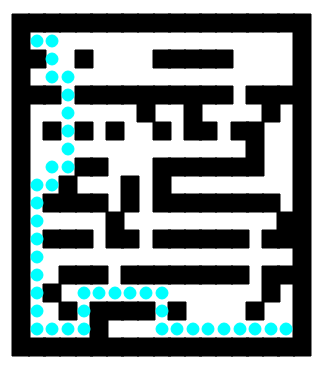
\includegraphics[width=0.46\textwidth]{NoOptSolution.png}
			
		\end{figure}

		\par
		La solución óptima encontrada por el segundo algoritmo, de tamaño 35, es:

		\vspace{5mm}

		\begin{figure}[h]

			\centering
			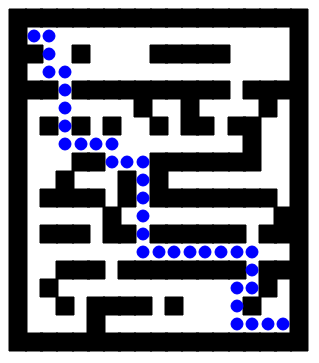
\includegraphics[width=0.46\textwidth]{OptSolutionBlue.png}
			
		\end{figure}

\newpage

	\section{Conclusión.}

		\par
		La técnica de \textit{Backtracking} permite explorar el espacio de soluciones de forma completa si uno lo desea, pero el coste de hacerlo puede ser demasiado alto. Hemos podido comprobar cómo el algoritmo encontraba soluciones óptimas, lo cual es una ventaja; sin embargo, para tamaños de entrada muy pequeños en comparación con otros algoritmos, \textit{Backtracking} comienza a ser inviable.

		\par
		En definitiva, deberíamos tener muy en cuenta la dimensión de nuestro problema antes de decidir resolverlo mediante este tipo de algoritmos, ya que la exploración sistemática no suele ser factible en la práctica.

\end{document}